\documentclass{article}
\usepackage{graphicx}
\usepackage{enumerate}
\usepackage{amsmath}
\usepackage{amsthm}
\usepackage{amsfonts}
\usepackage{hyperref}

\usepackage{amssymb}

\usepackage{amsmath}  

\usepackage{algorithm}  
\usepackage{algpseudocode}  
\usepackage{amsmath}  
\renewcommand{\algorithmicrequire}{\textbf{Input:}}  % Use Input in the format of Algorithm  
\renewcommand{\algorithmicensure}{\textbf{Output:}} % Use Output in the format of Algorithm    
\usepackage{listings}
\usepackage{url}

\usepackage{etoolbox}
\newtoggle{solution}
\toggletrue{solution}
%\togglefalse{solution}
\usepackage{color}
\newcommand{\solution}[2][0pt]{\iftoggle{solution}{\smallskip{\color{red}{\flushleft\textbf{Solution}:}\par#2}}{\vspace*{#1}}}

\renewcommand{\baselinestretch}{1.2}%Adjust Line Spacing
%\geometry{left=2.0cm,right=2.0cm,top=2.0cm,bottom=2.0cm}% Adjust Margins of the File

% Create horizontal rule command with an argument of height
\newcommand{\horrule}[1]{\rule{\linewidth}{#1}}
% Set the title here
\title{
    \normalfont \normalsize
    \textsc{ShanghaiTech University} \\ [25pt]
    \horrule{0.5pt} \\[0.4cm] % Thin top horizontal rule
    \huge CS240 Algorithm Design and Analysis \\ % The assignment title
    \LARGE Fall 2022\\
    \LARGE Problem Set 3\\
    \horrule{2pt} \\[0.5cm] % Thick bottom horizontal rule
}
% wrong usage of \author, never mind
\author{Dai ZiJia 2022233158}
\date{Due: 23:59, Nov. 24, 2022}

% Add the support for auto numbering
% use \problem{title} or \problem[number]{title} to add a new problem
% also \subproblem is supported, just use it like \subsection
\newcounter{ProblemCounter}
\newcounter{oldvalue}
\newcommand{\problem}[2][-1]{
	\setcounter{oldvalue}{\value{secnumdepth}}
	\setcounter{secnumdepth}{0}
	\ifnum#1>0
		\setcounter{ProblemCounter}{#1}
	\else
		\stepcounter{ProblemCounter}
	\fi
	\section{Problem \arabic{ProblemCounter}: #2}
	\setcounter{secnumdepth}{\value{oldvalue}}
}
\newcommand{\subproblem}[1]{
	\setcounter{oldvalue}{\value{section}}
	\setcounter{section}{\value{ProblemCounter}}
	\subsection{#1}
	\setcounter{section}{\value{oldvalue}}
}

\begin{document}
\maketitle
\vspace{3ex}

\begin{enumerate}
%\item Please write your solutions in English. 
\item Submit your solutions to Gradescope (www.gradescope.com).
\item In ``Account Settings'' of Gradescope, set your FULL NAME to your Chinese name and enter your STUDENT ID correctly. 
\item If you want to submit a handwritten version, scan it clearly. Camscanner is recommended. 
\item When submitting your homework, match each of your solution to the corresponding problem number. 
%\item Violations to any of above may result in some penalty on your score. 
\end{enumerate}

\newpage
\problem{}
Suppose there is a finite set \textit{C} and a collection of subsets of \textit{C}. The SET-PACKING problem asks if some K subsets in the collection are pairwise disjoint(in other words, no two of them share an element). Show that SET-PACKING problem is NP-complete.\\
Hint: Reduction from Independent Set.


\solution{
To show that SET-PACKING problem is NP-complete, we should prove that the solution can be verified in polynomial time first. Assume that we have $k$ subsets, if we want to check whether they are pairwise disjoint, we need to check $k^2$ times and each check cost no more than $O(n)$. In conclusion, the verification can be done in polynomial time and it's a NP problem.  

Then we need a polynomial-time reduction from Independent Set: Given a graph $G = (V,E)$ and a number $k$, we define that $S(v) \subset E$ as a family, which means for every node $v\in V$ it contains all edges adjacent with $v$. We define that $S(v)$ and $v$ is a group with center $v$, so two groups are disjoint if and only if their centers are not adjacent. Therefore, $G$ contains an independent set of $k$ nodes if and only if we can select $k$ pairewise disjoint sets from this family.

Finally, we need to show yes-instances of Independent Set map to yes-instances of Set-Packing:

->: Suppose there is an independent set problem on a graph $G(V,E)$, we create a collection of $C$ sets, and for $v \in V$ has a set $S_v \in C$ which contains all edges adjacent to $v$. So each set packing in $C$ matches a set of vertices no two of which have same edge. Therefore it is an independent set in $G$ of the same size.

<-: Suppose there is a set packing problem on a collection $C$, we create  a graph $G(V,E)$, where for every $S\in C$ has a vertex $v_S\in V$ and if $S_1,S_2$ intersect there is an edge between $v_{S_1},v_{S_2}$. So every independent set(vertex) in $G$ matches a set of sets from $C$ that no two of which intersect. 

From the above aspects, it's proved that SET-PACKING problem is NP-complete.
}

\newpage
\problem{}
Red and Xiaoyu are allocating a set of items $M=\{1,...,m\}$ among themselves. Each of them evaluates the items respectively and gives each of the items a valuation to
denote their preference on the item. Given a subset of items $S\subseteq M$, one's utility is defined as 
$$u_i(S)=max\{ \sum_{j\in S}v_i(j), b_i\}$$
where $i\in \{Red,Xiaoyu\}$, $v_i(j)$ is $i$'s valuation on item $j$ and $b_i$ is the upper bound of $i$'s utility. Their goal is to find the optimal allocation $S_1,S_2$ that maximizes $u_R(S_1)+u_X(S_2)$. Prove this problem is NP-hard with "Knapsack".

Here is an example for you to understand the problem. There are 3 items indexed by $1,2,3$. Red's valuation on the items are $10,20,30$ and Xiaoyu's valuation is $30,15,10$ while the upper bound of their total utilities are $40$ and $50$. Then the best choice is to allocate item $3$ to Red and $1,2$ to Xiaoyu which brings a $30 + ( 30 + 15)=75$ utility in total.

\solution{
To prove this problem is NP-hard, we need a polynomial time reduction Knapsack $\le_p$ this problem.

The knapsack problem determine the number of each item to include in a collection so that the total weight is less than or equal to a given limit and the total value is as large as possible, it's shown below:
$$maxmize\sum^n_{i=1}v_ix_i$$ 
$$s.t.\sum^n_{i=1}w_ix_i \le W, x_i\in \{0,1\}$$

1. Suppose there is an instance $S$, which is a subset of items $S\subseteq M$. We can reconstruct the problem in polynomial time as knapsack's input size:
$$v_{Red}(j) = \frac{v_j}{V}$$
$$v_{Xiaoyu}(j) = w_j$$
$$b_{Red} = \sum_{j=1}^n \frac{v_j}{2V}$$
$$b_{Xiaoyu} = \sum_{j=1}^n w_j -W$$
$V$ is the maximum of all items, $W$ is the capacity of knapsack. The problem turns to:
$$\max_S(u_{Red}(S)+u_{Xiaoyu}(M-S))$$ 

2. If $S$ is optimal for the problem, it would then yield a solution to knapsack. For the reason:
$$\max_S(u_{Red}(S)+u_{Xiaoyu}(M-S)) = \max_S(\sum_{i \in S}\frac{v_j}{V}+\sum_{j=1}^n w_j -W)$$
$$\Leftrightarrow \max_S\sum_{i \in S}v_j$$

From the above aspects, it proves the problem is NP-Hard because if we know how to solve the problem then we know how to solve “knapsack” and since “knapsack” is NP-Hard then automatically the problem must be NP-hard.
}

\newpage
\problem{}
The problem: Suppose there is an undirected graph $G= (V, E)$ and a positive integer $M \leq |V|$. Does the gragh $G$ contain a path which   visits vertex at most once and has the number of path's edges $N \geq M$ ?
\newline
Prove this problem is NP-complete.

\solution{
To show the problem is NP-complete, we should prove that the solution can be verified in polynomial time first. The certification would be a list of vertices $\{v_1,v_2..,v_M\}$ in order of the path. We can check in polynomial time whether $\{ v_i,v_{i+1}\}$ is an edge($1\le i\le N-1$). Thus, it's a NP problem. 

Then we reduce Hamiltonian path to this problem: Given a graph $G(V,E)$ with an instance of undirected Hamiltonian path $P$, according to thr defination it must visits each vertex exactly once, the problem path will equal to the path $P$ when integer $M < |V|$, which satisfies visiting vertex at most once and has the number of path's edges $N \ge M$.

Finally, we need to show yes-instances of Hamiltonian path map to yes-instances of problem path:

->: Suppose $G(V,E)$ has an instance of undirected Hamiltonian path $P$, $P$ will be the problem path when integer $M < |V|$ too.

<-:  Suppose $G(V,E)$ has an instance of the problem path $P$, $P$ will be Hamiltonian path when integer $M = |V|-1$ too.

From the above aspects, it's proved that this problem is NP-complete.
}

\newpage
\problem{}
STINGY SAT is the following problem: given a set of clauses (each a disjunction of literals) and an integer k, find a satisfying assignment in which at most k variables a true, if such an assignment exists. Prove that STINGY SAT is NP-complete.

\solution{
It's obvious that the verification of sting SAT can be done in polynomial time beacuse we just need to verify $k$ clause and it's a NP problem.  

Then we need a polynomial-time reduction from SAT: Given a SAT $A$, assume that $(A,k)$ is a sting SAT where $k$ equals to the number of variables in SAT $A$.

Finally, we need to show yes-instances of SAT map to yes-instances of sting SAT:

->: Suppose $A$ has a truth $T$. Because $A$ has $k$ variables, $T$ will be a positive solution for sting SAT $(A,k)$ too.

<-: Suppose $(A,k)$ has a truth $T$ and no more than $k$ variables shows true. Apparently $T$ is a positive solution for SAT $A$ too.

From the above aspects, it's proved that sting SAT problem is NP-complete.
}

\newpage
\problem{}

SIST allows students to work as TAs but would like to avoid TA cycles. A TA cycle is a list of TAs ($A_{1}$, $A_{2}$, . . . , $A_{k}$) such that $A_{1}$ works as a TA for $A_{2}$ in some course, $A_{2}$ works as a TA for $A_{3}$ in some course, · · · , and finally $A_{k}$ works as a TA for $A_{1}$ in some course. We say a TA cycle is simple if it does not contain the same TA more than once. Given the TA arrangements of SIST, we want to find out whether there is a simple TA cycle containing at least K TAs. Prove this problem is NP-complete.

\solution{
To show that TA cycle problem is NP-complete, we should prove that the solution can be verified in polynomial time first. Assume that we have $k$ TAs, if we want to check whether they can be a TA cycle, one counts the vertices to make sure they are all there, then checks that each is connected to the next by an edge, and whether the last is connected to the first which takes time proportional to $O(k)$. $O(k)$ is a polynomial, so the check runs in polynomial time. In conclusion, the verification can be done in polynomial time and it's a NP problem.
	
Then we need a polynomial-time reduction from 3-SAT: Suppose there is variables set $U = \{x_1,..,x_n\}$, it's nagation is $\overline{U} = \{\neg x_1,..,\neg x_n\}$. $B = C_1\wedge...\wedge C_m$ is a boolean expression, where $C_i = (\alpha \vee \beta \vee \gamma),\alpha,\beta,\gamma \in U \cup \overline{U}$. 
\begin{itemize}
	\item For each variable $x_i\in U$, create vertices $c_{i,1},...,c_{i,3(m+1)}$, add $s,t$. Create edges $s\to c_{1,1},c_{1,3(m+1)}$; $c_{n,1},c_{n,3(m+1)}\to t$; for each $c_{i,j}\rightleftharpoons c_{i,j+1}$; $c_{i,1},c_{i,3(m+1)}\to c_{i+1,1},c_{i+1,3(m+1)}$.
	\item For each clause $C_i$, create a vertex. If $x_j$ appears in $C_i$ create edges $c_{j,3i}\rightleftharpoons C_i$ and $C_i \rightleftharpoons c_{j,3i+1}$. If $\neg x_i$ appears in $C_i$ create edges $c_{j,3i+1}\rightleftharpoons C_i$ and $C_i \rightleftharpoons c_{j,3i}$. 
\end{itemize}
\begin{figure}[ht]
	\centering
	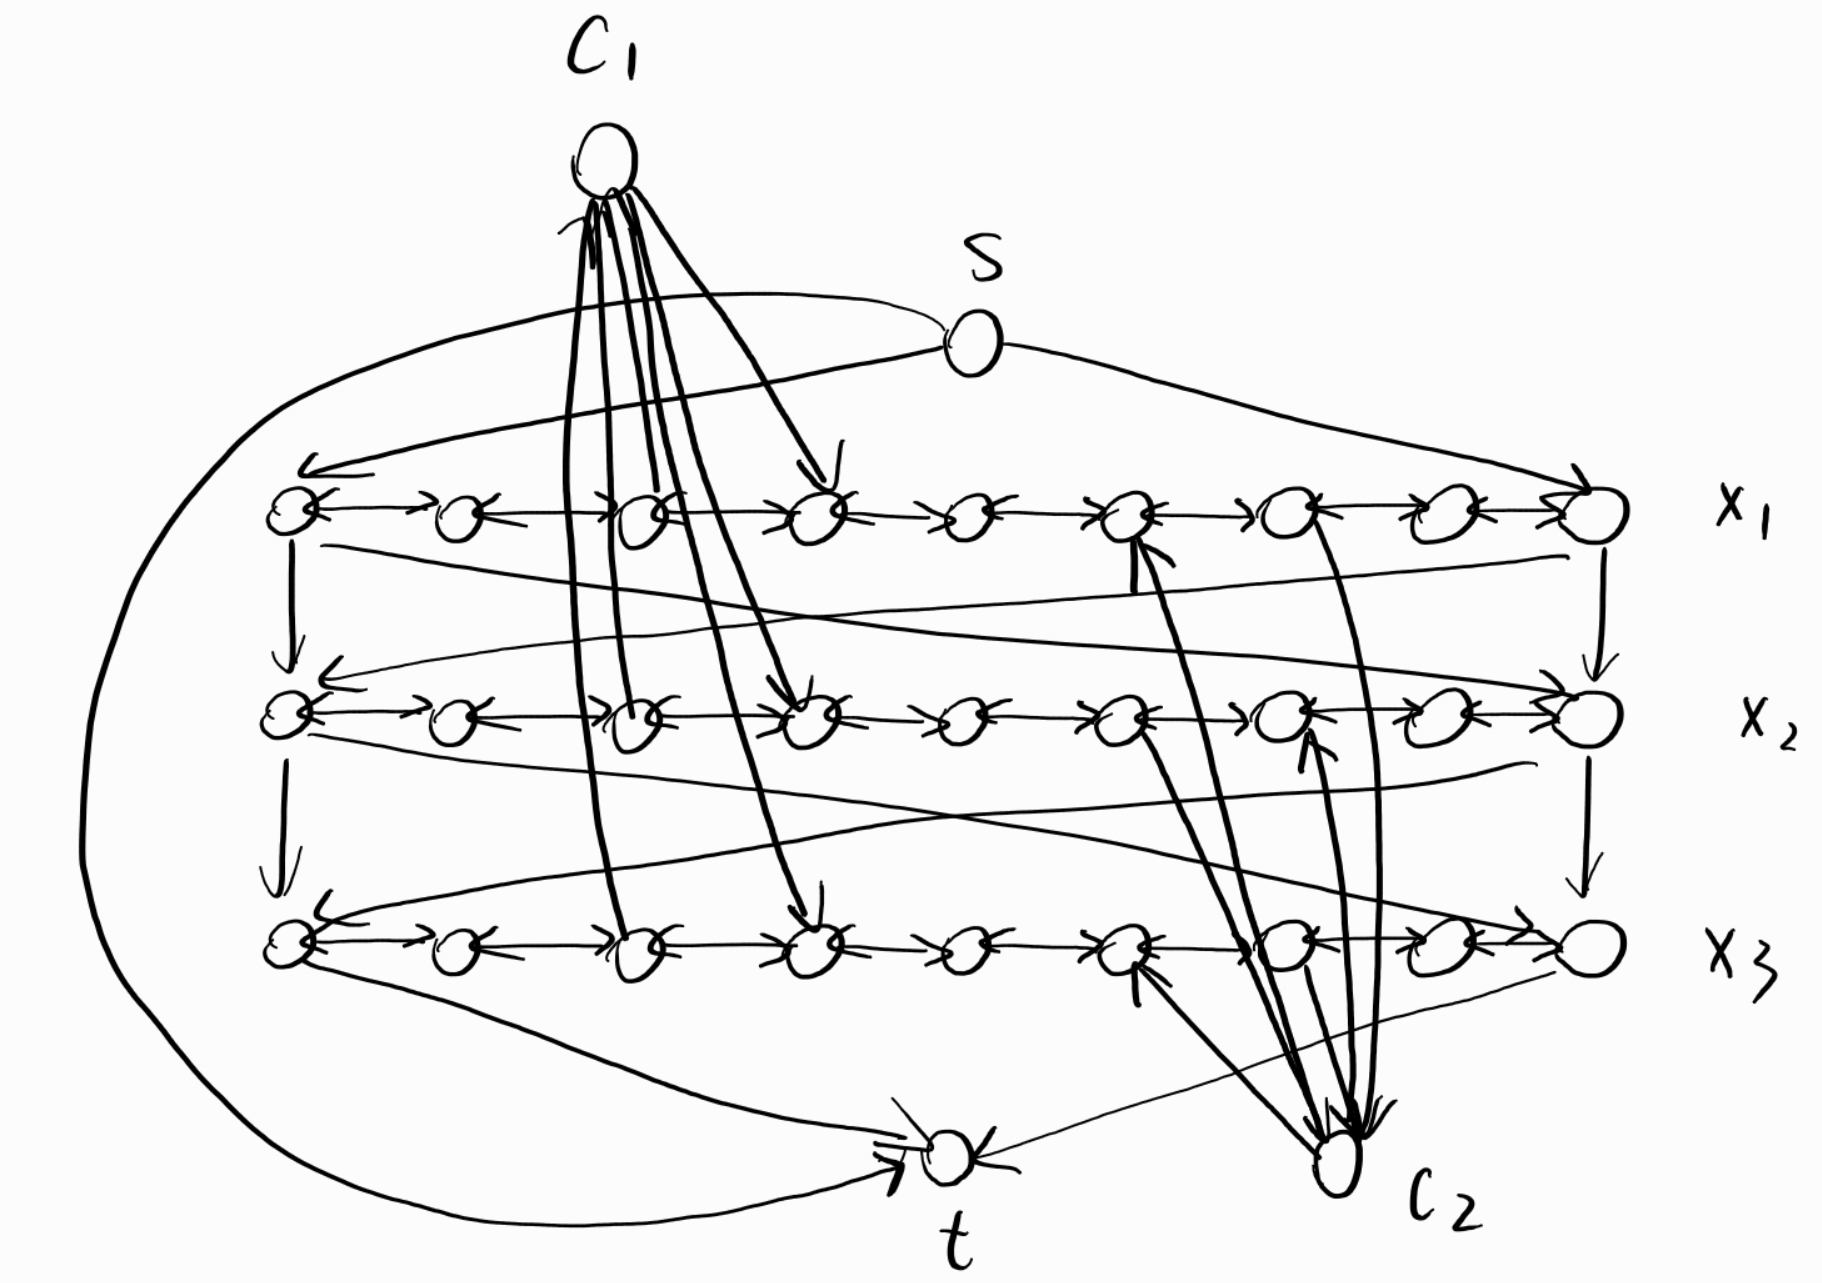
\includegraphics[scale=0.2]{q5.jpg}
	\caption{The graph from $B$.}
\end{figure}

It's easy to know that the graph contains $2+m+3(m+1)n$ vertices and $2mn+3m+5$ edges, which is constructed in polynomial time. Finally, we need to show yes-instances of 3-SAT map to yes-instances of TA cycle problem:

->: Suppose $T$ is a truth that satisfies $B$. Begin at $s$, go to $c_{1,1}$ or $c_{1,3(m+1)}$ for $x_1$ is true or false. Go along the row and may go through $C_i$ if it's available. Then go to $c_{2,1}$ or $c_{2,3(m+1)}$ if $x_2$ is true or false and continue. There will be at least one route to go through each $C_i$, and the path will visit every vertex of $G$. Therefore, we can find a TA cycle of $G$ when there is a satisfying truth assignment.

<-: Suppose $H$ is a TA cycle(Hamiltonian circuit) on $G$. It starts at $s$ and must go either $c_{1,1}$ or $c_{1,3(m+1)}$. Assume that $x_i$ is true if $H$ go to $c_{1,1}$ and false go to $c_{1,3(m+1)}$, continue to go through $x_2,..,x_n$, at last arrive $t$ to finish. It's known to us that each $C_i$ is traversed, which means each $C_i$ contains a $x_i$ or $\neg x_i$($x_i$ is boolean). Therefore, we can find a satisfying truth assignment when there is a TA cycle.

From the above aspects, it's proved that TA cycle problem is NP-complete.

}


\end{document}
